\documentclass[a4paper,11pt,fleqn]{article}%fleqn pour aligner les equations à gauche
\usepackage{../../Styles/Cours}


\newcommand{\chnum}{Chapitre 1}
\newcommand{\chtitle}{L'abondance des éléments chimiques dans l'Univers}
\newcommand{\dtype}{Act 1}


\begin{document}
\maketitle
Dans l'Univers, il existe plus d'une centaine d'éléments chimiques différents. Ces noyaux d'éléments sont répartis dans des proportions différentes entre les étoiles, la Terre ou les êtres vivants. \textbf{Comment les éléments chimiques sont-ils répartis dans l'Univers ?}

\begin{figure}[h!]
    \begin{minipage}{.48\linewidth}
    \caption{\textbf{La formation des premiers noyaux}}
    Quelques secondes après le Big Bang, les particules élémentaires ont formé les premiers noyaux d'atomes d'hydrogène \ce{H}, d'hélium \ce{He} et de lithium \ce{Li}.\\
    Ces noyaux ont ensuite fusionné pour former de nouvelles variétés isotopiques d'hydrogène (le deutérium $_1^2H$ et le tritium $_1^3H$), l'hélium 3 et 4, le lithium 6 et 7, ainsi que le béryllium 7. Cette première étape est appellée \textit{nucléosynthèse primordiale}.\\
    Environ 300 secondes après le Big Bang, la température et la densité sont devenues trop faibles pour maintenir les conditions de la \textit{nucléosynthèse primordiale} qui s'est alors interrompue.
    \end{minipage}\hspace{.04\linewidth}
    \begin{minipage}{.48\linewidth}
        \caption{\textbf{La formation des noyaux lourds}}
        Après la nucléosynthèse primordiale, les noyaux légers se sont rassemblés et ont commencé à former des noyaux plus lourds au sein des étoiles : ce processus est appelé \textit{nucléosynthèse stellaire}.\\
        La fusion des noyaux d'atomes d'hydrogène a permis, entre autres, la formation d'hélium 4.\\
        D'autres réaction se sont produites par la suite et les noyaux atomiques plus lourds (jusqu'au fer $Z=26$) sont apparus au coeur des étoiles.\\
        Au fur et à mesure des fusions, une étoile gagne en masse, ce qui entraine à terme son éfondrement sous l'effet de l'interaction gravitationnelle. Lors de cet effondrement, les couches externes de l'étoile sont expulsées. De nouvelles réactions de fusion sont alors mises en route permettant la formation de noyaux encore plus lourds ($Z>26$). C'est la \textit{nucléosynthèse explosive}.
        \end{minipage}
\end{figure}

\begin{figure}[h!]
    \begin{minipage}{.48\linewidth}
    \caption{\textbf{Les éléments chimiques dans l'Univers}}
    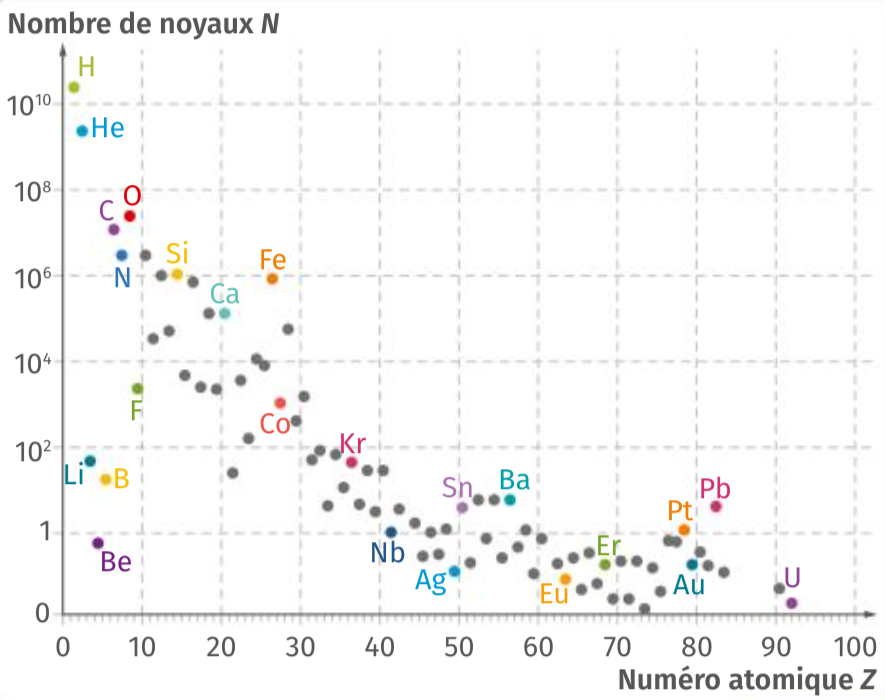
\includegraphics[width=\linewidth]{Ressources/1ES_Act1_Fig1.png}\\
    On connait 118 éléments chimiques à ce jour mais leur \textit{abondance relative} est très variable. Sur ce graphique, $N$ représente le nombre de noyaux d'un élément chimique dont le numéro est $Z$, en les comparant à une population de référence de $10^6$ noyaux de silicium \ce{Si}.
    \end{minipage}\hspace{.04\linewidth}
    \begin{minipage}{.48\linewidth}
    \caption{\textbf{Nébuleuse}}
    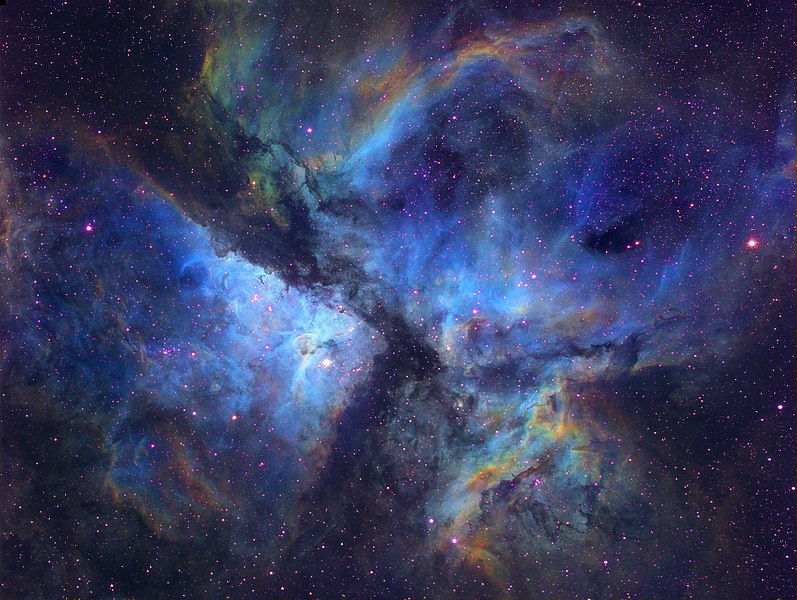
\includegraphics[width=\linewidth]{Ressources/nebuleuse.jpeg}\\
    L'expulsion des couches externes des étoiles massives forment des nébuleuses où l'on peut retrouver des éléments lourds.
    \end{minipage}
\end{figure}

\begin{figure}[h!]
    \begin{minipage}{.48\linewidth}
    \caption{\textbf{L'abondance relative des éléments chimiques dans le monde vivant}}
    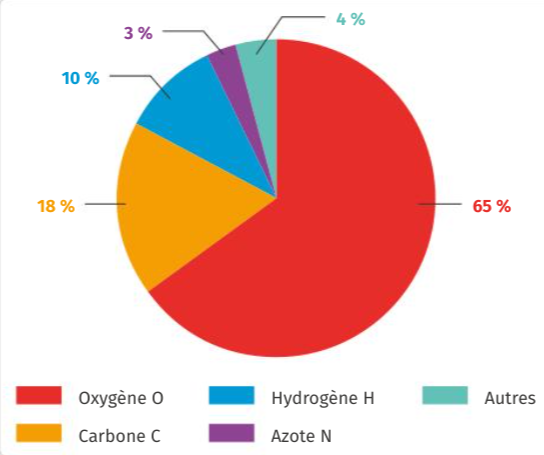
\includegraphics[width=\linewidth]{Ressources/1ES_Act1_Fig2.png}
    \end{minipage}\hspace{.04\linewidth}
    \begin{minipage}{.48\linewidth}
    \caption{\textbf{L'abondance massique des éléments chimique sur le sol lunaire}}
    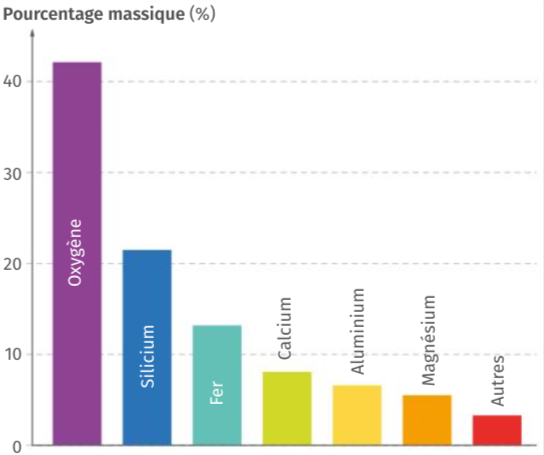
\includegraphics[width=\linewidth]{Ressources/1ES_Act1_Fig3.png}
    \end{minipage}
\end{figure}

\begin{figure}[h!]
    \begin{minipage}{.48\linewidth}
    \caption{\textbf{L'abondance massique des éléments chimiques dans la croûte terrestre}}
    \begin{tabular}{|m{.45\linewidth}|m{.45\linewidth}|}

        \hline
        \textbf{Élément} & \textbf{Pourcentage massique}\\ \hline
        Oxygène \ce{O} ($Z=8$) & \SI{46}{\percent}\\ \hline
        Silicium \ce{Si} ($Z=14$) & \SI{28}{\percent}\\ \hline
        Aluminium \ce{Al} ($Z=13$) & \SI{8}{\percent}\\ \hline
        Fer \ce{Fe} ($Z=26$) & \SI{6}{\percent}\\ \hline
        Calcium \ce{Ca} ($Z=20$) & \SI{4}{\percent}\\ \hline
        Autres & \SI{8}{\percent}\\ \hline
    \end{tabular}
    \end{minipage}\hspace{.04\linewidth}
    \begin{minipage}{.48\linewidth}
    \caption{\textbf{L'abondance massique des éléments chimique dans la photosphère du Soleil}}
    \begin{tabular}{|m{.45\linewidth}|m{.45\linewidth}|}

        \hline
        \textbf{Élément} & \textbf{Pourcentage massique}\\ \hline
        Hydrogène \ce{H} ($Z=1$) & \SI{73,46}{\percent}\\ \hline
        Hélium \ce{He} ($Z=2$) & \SI{24,85}{\percent}\\ \hline
        Oxygène \ce{O} ($Z=8$) & \SI{0,77}{\percent}\\ \hline
        Carbone \ce{C} ($Z=6$) & \SI{0,29}{\percent}\\ \hline
        Fer \ce{Fe} ($Z=26$) & \SI{0,16}{\percent}\\ \hline
        Néon \ce{Ne} ($Z=10$) & \SI{0,12}{\percent}\\ \hline
        Autres & \SI{0,35}{\percent}\\ \hline
    \end{tabular}
    \end{minipage}
    Le Soleil est un astre dans lequel on trouve principalement de l'hydrogène \ce{H} et de l'hélium \ce{He}. Il contient aussi d'autres éléments chimiques, dont les proportions sont beaucoup plus faibles. En astrophysique, tous les éléments chimiques de numéro atomiques $Z$ supérieurs à 2 est considéré comme des "éléments lourds".
\end{figure}

\noindent\begin{minipage}{\linewidth}
    \textbf{Questions :}
    %\begin{multicols}{2}
        \begin{enumerate}
            \item Décrire les principales étapes de la formation des éléments chimiques dans l'Univers. \textcolor{gray!80!blue}{\textbf{Doc. 1 et 2}}
            \item Identifiez les deux éléments chimiques les plus abondants dans l'Univers. Combien de fois sont-ils plus repésents que le silicium (\ce{Si}) d'après les abondances fournies ? \textcolor{gray!80!blue}{\textbf{Doc. 3}}
            \item Réaliser des diagrammes circulaires de l'abondance massique des éléments dans la croûte terrestre et sur le sol lunaire. \textcolor{gray!80!blue}{\textbf{Doc. 5 et 6}}
            \item Réaliser un diagramme en bâtons empilés comparant l'abondance massique des éléments chimiques dans le monde vivant, la croûte terrestre, le sol lunaire et la photosphère du Soleil.
        \end{enumerate}
    %\end{multicols}
\end{minipage}
\end{document}


\begin{figure}[h!]
    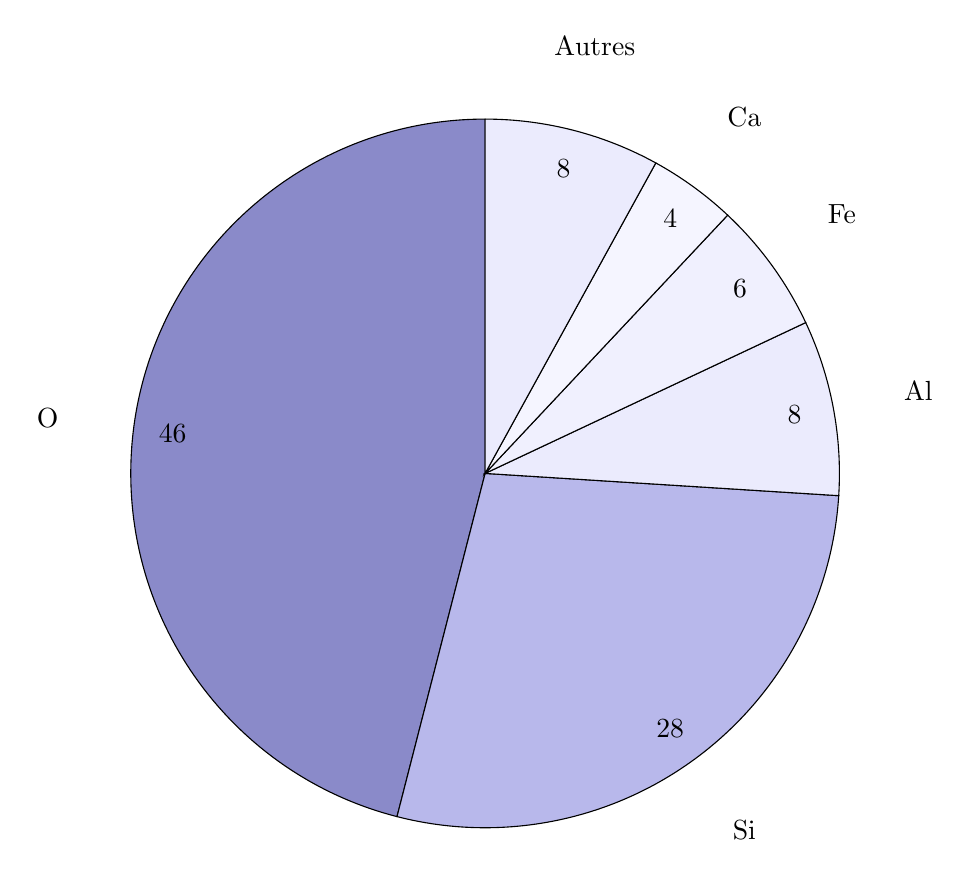
\begin{tikzpicture}
        \foreach \a/\b/\p/\c in
            {90/255.6/46/O, 255.6/356.4/28/Si, -3.6/25.2/8/Al, 25.2/46.8/6/Fe, 46.8/61.2/4/Ca, 61.2/90/8/Autres}
            {
                \draw[fill=black!\p!blue!\p]
                    (0,0) -- (\a:4.5) arc (\a:\b:4.5) -- cycle;
                \draw ({(\a+\b)/2}:4) node {\p};
                \draw ({(\a+\b)/2}:5.6) node {\c};
            }

    \end{tikzpicture}
    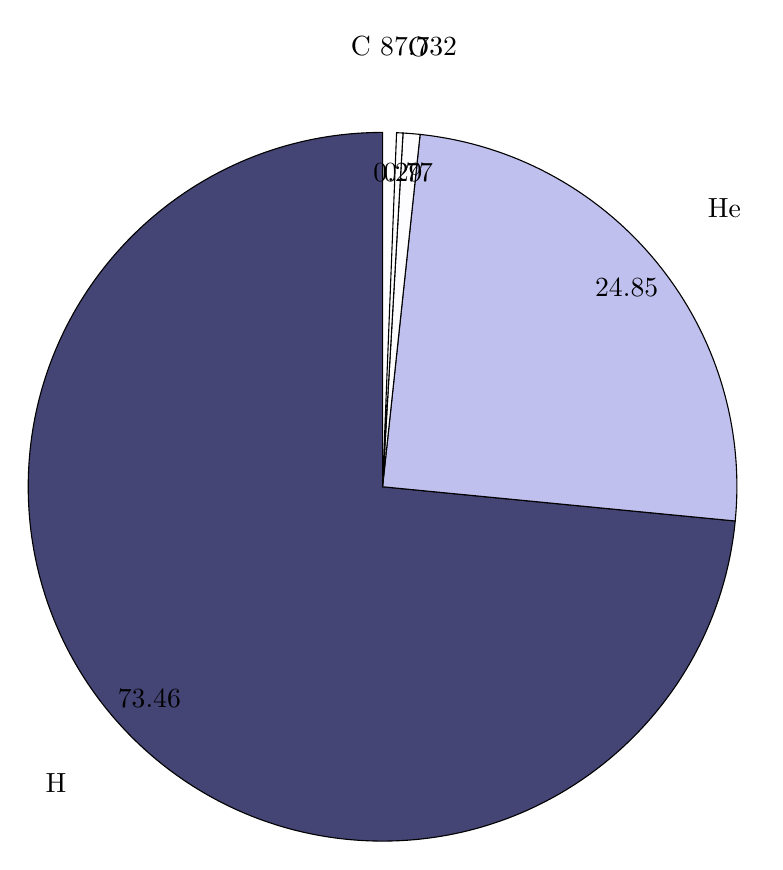
\begin{tikzpicture}
        \foreach \a/\b/\p/\c in
            {90/354.456/73.46/H, -5.544/83.916/24.85/He, 83.916/86.688/0.77/O,
            86.688/87.732/0.29/C
            87.732/88.308/0.16/Fe
            88.308/88.74/0.12/Ne
            88.74/90/0.35/Autres
            }
            {
                \draw[fill=black!\p!blue!\p]
                    (0,0) -- (\a:4.5) arc (\a:\b:4.5) -- cycle;
                \draw ({(\a+\b)/2}:4) node {\p};
                \draw ({(\a+\b)/2}:5.6) node {\c};
            }

    \end{tikzpicture}  
\end{figure}
